\documentclass{beamer}

\usepackage{udesc}
\usepackage{graphicx,url}
\usepackage{multicol}
\usepackage{hyperref}
\usepackage{caption}
\usepackage[utf8]{inputenc}
%\usepackage[T1]{fontenc}
\usepackage{booktabs}
\usepackage[brazil]{babel}

\title[Paladar - Interfaces Gustativas]{Paladar - Interfaces Gustativas}

\author[Dalton Solano dos Reis]{
  Dalton Solano dos Reis\texorpdfstring{\\\medskip}{}%
  {\small \href{mailto:dalton@furb.br}{dalton@furb.br}}}

\institute[UDESC]{
  % Departamento de Ciêcia da Computação \\
  Centro de Ciências e Tecnológicas\\
  Universidade do Estado de Santa Catarina}

\begin{document}

\begin{frame}
  \titlepage

\end{frame}

\section{Pesquisa}
\begin{frame}
  \frametitle{Enunciado}
  \begin{itemize}
    \item Dalton S. dos Reis: \textbf{Paladar}
    \item Luciana P. A. Kohler: Olfato (relação forte com o \textbf{Paladar})  
    \item Nathália Miranda: OUTPUT-5. Other Senses
    \begin{itemize}
      \item a. Fone de Ouvido Háptico - Razer - Nari Ultimate, 2018
      \item b. Olfato
      \item \textbf{c. Paladar}  
    \end{itemize} 
  \end{itemize}
  A experiência gustativa (\textbf{Paladar}) humana envolve também:
  \begin{itemize}
    \item olfato
    \item textura
  \end{itemize}
\end{frame}

\begin{frame}
  \frametitle{Livro}
  Introdução a Realidade Virtual e Aumentada, 2020. \\
  \begin{itemize}
    \item Pag. 52: \textbf{paladar} alvo de investigações e produtos inovadores
    \item Pag. 153: A sensibilidade, o odor e o \textbf{paladar} estão longe de ser experimentados. Essas são as buscas dos cientistas das próximas gerações
    \item Pag. 191: olfato e \textbf{paladar} ainda não são pesquisados amplamente
    \item Pag. 407: maior interação quando se utiliza acessórios para aumentar a percepção (\textbf{paladar})
  \end{itemize}
  \begin{flushright}
    \scriptsize
    \cite{toriIntroducaoRealidadeVirtual2020}
  \end{flushright}
\end{frame}

\section{Conceitos}
\begin{frame}
  \frametitle{Visão geral}
  Existem dispositivos experimentais de \textbf{paladar} para Realidade Virtual (VR), mas ainda estão em estágios iniciais de desenvolvimento e não são amplamente disponíveis como os dispositivos visuais, auditivos ou táteis (hápticos) \\
  \vspace{\baselineskip}
  Dois grupos (sentidos):
  \begin{itemize}
  \item visão, audição e tato
  \item olfato e palar
  \end{itemize}
\end{frame}

\begin{frame}
  \frametitle{Dispositivos de paladar: métodos}
  \begin{itemize}
    \item Estimulação elétrica da língua
    \begin{itemize}
      \item eletrodos na língua para estimular os receptores gustativos
      \item simular sensações como azedo, salgado, doce ou metálico
    \end{itemize}
    \item Estimulação térmica
    \begin{itemize}
      \item mudanças de temperatura: afetam a percepção do sabor
      \item calor e frio para simular (picante ou refrescante)  
    \end{itemize}
    \item Sprays ou cartuchos de aroma e gosto
    \begin{itemize}
      \item dispositivos liberam aromas ou microgotas com sabor
      \item pode ser acoplado a fones de ouvido ou óculos VR
    \end{itemize}
    \item Realidade gustativa combinada
    \begin{itemize}
      \item RA com alimentos reais: comer algo neutro (biscoito sem sabor), enquanto o sistema altera visualmente e aromaticamente o alimento, convencendo o cérebro de que é algo diferente
    \end{itemize}
  \end{itemize}
\end{frame}

\section{Dispositivos}
\begin{frame}
  \frametitle{Exemplos de dispositivos}
  Dispositivos encontrados:
  \begin{multicols}{2}
    \begin{itemize}
      \item \textbf{Digital Lollipop}
      \item \textbf{Vocktail}
      \item Project Nourished
      \item e-Taste
      \item Meta Cookie+
      \item Thermal Taste Actuator
      \item Taste Display Synthesizer
      \item AR Taste Enhancers
      \item Mixed Reality Kitchen
      \item Virtual Sweet Spoon
      \item Electric Taste Machine
      \item Taste+ Project
      \item Augmented Gustation
      \item Multisensory XR System
    \end{itemize}
  \end{multicols}  
  \begin{flushright}
    \scriptsize
    14 hardwares
  \end{flushright}
\end{frame}

\begin{frame}
  \frametitle{Digital Taste Interface (DTI) - Digital Lollipop}
  \begin{itemize}
    \item Nimesha Ranasinghe - Universidade de Singapura
    \item Ano: 2013 (protótipo inicial)
    \item Método: estimulação elétrica  e térmica da Língua
    \item Sabores: doce, salgado, azedo e amargo
    \item Aplicações:
    \begin{itemize}
      \item entretenimento
      \item auxiliar pessoas com restrições alimentares (diabéticos - simular sabores sem a ingestão real de açúcar)
    \end{itemize}
    \item Dispositivo: eletrodos de prata na ponta da língua para aplicar correntes elétricas de baixa intensidade, com variações de magnitude, frequência e polaridade
    \item Explora: Taste Over Internet Protocol (\textbf{TOIP})
    \begin{itemize}
      \item transmitir informações gustativas digitalmente entre locais
    \end{itemize}
  \end{itemize}
  \begin{flushright}
    \scriptsize
    \cite{ranasingheTongueMountedInterface2012}
    \cite{ranasingheVirtualTasteDigital2023}
  \end{flushright}
\end{frame}

\begin{frame}
  \frametitle{Digital Taste Interface (DTI) - Digital Lollipop}
  \begin{figure}[h]
    \centering
    \caption{Dispositivo Digital Lollipop}
    \vspace{-18pt}
    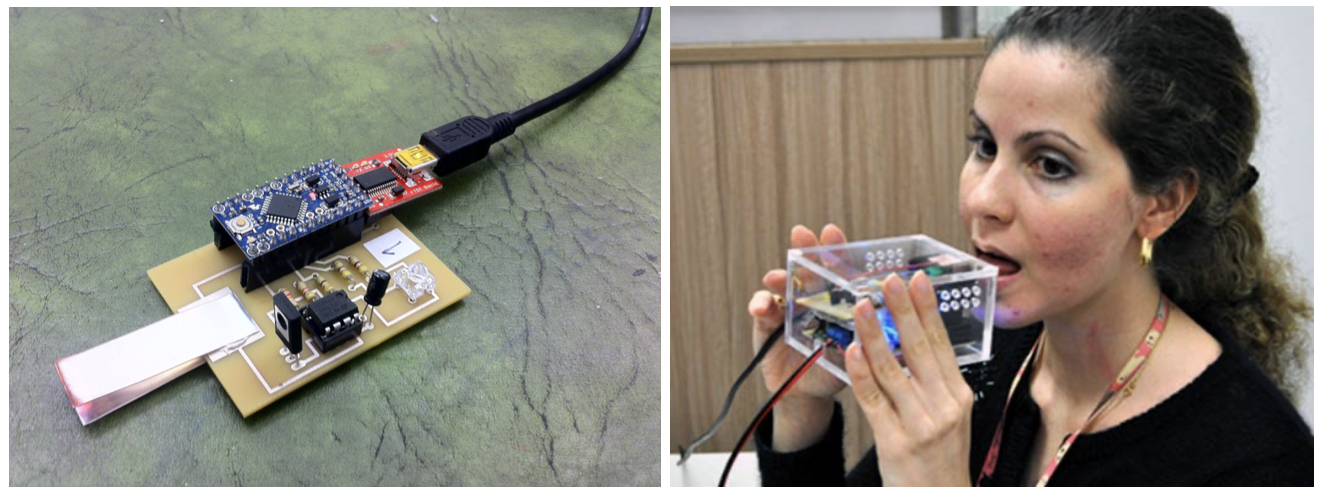
\includegraphics[width=1.03\textwidth]{img_DigitalLollipop.png}
    \vspace{-20pt}
    \caption*{Fonte: \cite{ranasingheDigitalLollipopStudying2016}.}
  \end{figure}
\end{frame}

\begin{frame}
  \frametitle{Vocktail (Virtual Cocktail)}
  \begin{itemize}
    \item desenvolvido: Ranasinghe (Keio-NUS CUTE Center - 2017)
    \item taça com uma base impressa 3D (componentes eletrônicos)
    \item dispositivo interativo: aplicativo móvel via Bluetooth
    \item usuários personalizem as combinações de sabor, aroma e cor
    \item simula água simples seja percebida como um coquetel
    \item estímulos sensoriais para criar sabores virtuais:
    \begin{itemize}
      \item visual: LEDs RGB - luzes coloridas influenciando o sabor
      \item gustativo: eletrodos de prata na borda: salgado/azedo/amargo
      \item olfativo: microbombas de ar liberam aromas de cartuchos
    \end{itemize}
  \end{itemize}
\end{frame}

\begin{frame}
  \frametitle{Vocktail}
  \begin{figure}[h]
    \centering
    \caption{Exemplo do Vocktail}
    \vspace{-8pt}
    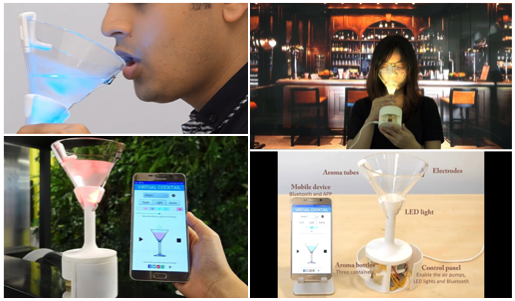
\includegraphics[width=0.7\textwidth]{../Vocktail.png}
  \end{figure}
\end{frame}

% \begin{frame}
%   \frametitle{Project Nourished}
%   \begin{itemize}
%     \item Jinsoo An e equipe
%     \item Método: realidade gustativa combinada
%     \item Funcionamento:
%     \begin{itemize}
%       \item  alimentos comestíveis de baixa caloria impressos em 3D
%       \item difusores de aromas e utensílios com sensores
%       \item simulações em VR
%     \end{itemize}
%     \item Exemplo:
%     \begin{itemize}
%       \item gelatina neutra pode ser percebida como uma torta de maçã ao combinar estímulos visuais, olfativos e táteis
%     \end{itemize}
%   \end{itemize}
% \end{frame}

% \begin{frame}
%   \frametitle{Project Nourished}
%   \begin{figure}[h]
%     \centering
%     \caption{Exemplo do Projeto Nourished}
%     \vspace{-8pt}
%     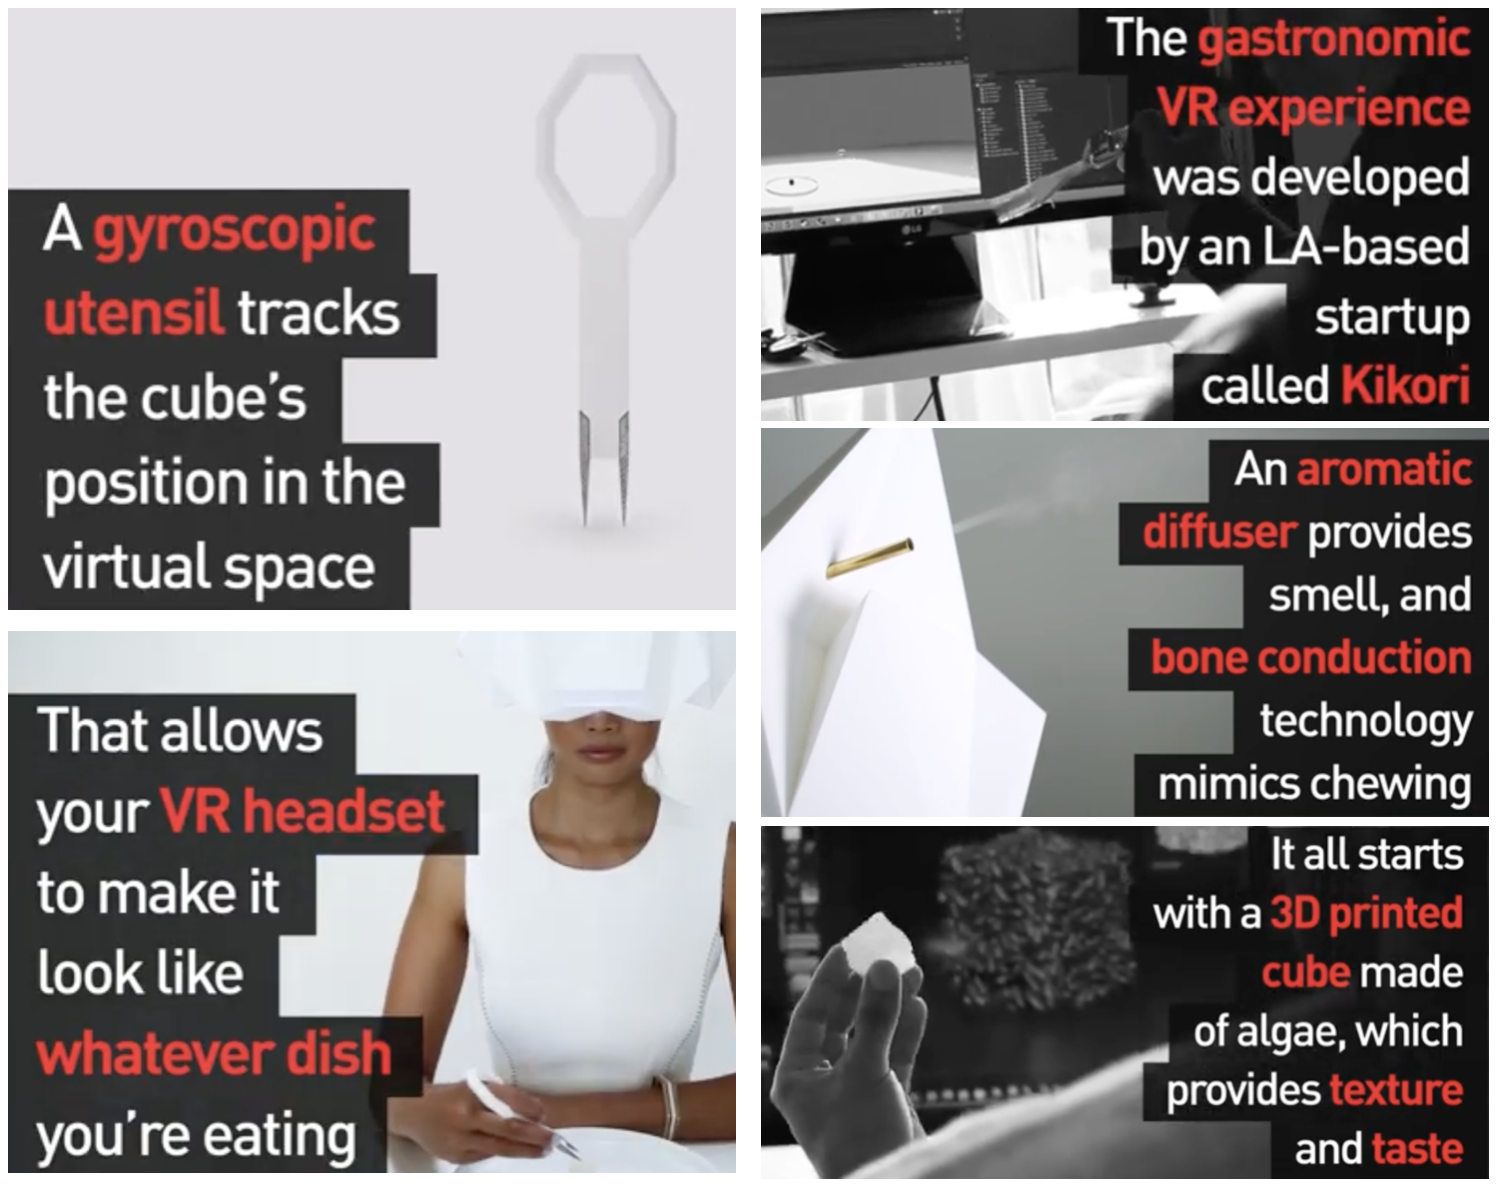
\includegraphics[width=0.7\textwidth]{img_ProjectNourished.png}
%   \end{figure}
% \end{frame}

\section{Situação atual}
\begin{frame}
  \frametitle{Situação atual}
  Dispositivos ainda está em fase de protótipo ou pesquisa \\
  \begin{itemize}
    \item Interfaces Gustativas Portáteis
    \begin{itemize}
      \item pirulito que utilizam hidrogéis
      \item substâncias químicas comestíveis
      \item de 2 a 9 sabores diferentes (iontoforese)
      \item ajustes na intensidade do sabor conforme a voltagem aplicada
    \end{itemize}
    \item Desafios:
    \begin{itemize}
      \item acesso: segurança e higiene
      \item padronização dos sabores
      \item garantia de segurança: substâncias químicas
      \item miniaturização
      \item sincronização multissensorial: experiências imersivas
    \end{itemize}
    \item \cite{reisTrabalho4Interfaces2025}
  \end{itemize}
\end{frame}


% \section{Referências}
% \begin{frame}
%   \frametitle{Referências pesquisadas}
%   \begin{itemize}
%     \item \cite{ranasingheDigitalLollipopStudying2016}
%     \item \cite{ranasingheTongueMountedInterface2012}
%     \item \cite{ranasingheVirtualTasteDigital2023}
%     \cite{toriIntroducaoRealidadeVirtual2020}
%   \end{itemize}
% \end{frame}

\begin{frame}
  \frametitle{Referências}
  \begingroup
  \footnotesize
    \bibliographystyle{sbc}
    \bibliography{../../UDESC_RV}
  \endgroup
\end{frame}

\end{document}
